% ---
% titre: 9P - Figures géométriques planes
% theme: ES
% chapitre: Figures géométriques planes
% sous_chapitre:
% niveau: [9e]
% type: PLANIF
% tags: [c-figures-planes,c-angles,c-triangles,c-quadrilateres,c-constructions]
% source: latex
% ---

\header{Figures géométriques planes - Objectifs}

\def\arraystretch{1.2}
\begin{tabularx}{\linewidth}{|>{\centering\arraybackslash}p{3cm}|>{\centering\arraybackslash}p{3cm}|X|}
\hline
\cellcolor{themeColor!30} Livre & \cellcolor{themeColor!30} Fiches & \cellcolor{themeColor!30} \hfill Aide-mémoire\hfill\null\\
\hline
\multirow{4}{*}{pp. 107-127}&\multirow{4}{*}{pp. 103-141}&Figures géométriques planes : pp. 104-114\\
&&Angles : pp. 115-123\\
&&Triangles : pp. 128-130\\
&&Quadrilatères : pp. 137-139\\
\hline
\end{tabularx}
\def\arraystretch{1}


\def\arraystretch{1.6}
\begin{tabularx}{\textwidth}{|>{\raggedright\arraybackslash}X|>{\raggedright\arraybackslash}X|}
\hline
\cellcolor{themeColor!30}Compétences visées & \cellcolor{themeColor!30}Utilité dans la vie de tous les jours \\
\hline
Mobiliser les savoirs, savoir-faire et savoir être pour résoudre des problèmes en lien avec les figures géométriques. 
&\vspace{-1em}
\begin{itemize}[leftmargin=*, itemsep=2pt, topsep=0pt, partopsep=0pt, parsep=0pt, label=$\triangleright$]
     \item Construire un meuble
    \item Agencer un appartement
    \item Réaliser un dessin ou un croquis
    \item Lire un plan ou une carte
    \item Poser un carrelage ou un parquet
\end{itemize} \\
\hline

Développer des stratégies de recherche afin de résoudre des problèmes.
&\vspace{-1em}
\begin{itemize}[leftmargin=*, itemsep=2pt, topsep=0pt, label=$\triangleright$]
    \item Découper un projet en sous-tâches
    \item Choisir l'ordre des tâches à effectuer
\end{itemize} \\
\hline

Présenter sa démarche de façon claire (explications, grandeur cherchée, unités, calculs, réponse).
&\vspace{-1em}
\begin{itemize}[leftmargin=*, itemsep=2pt, topsep=0pt, label=$\triangleright$]
    \item Collaborer avec d'autres personnes
    \item Expliciter sa compréhension d'un sujet
    \item Argumenter
\end{itemize} \\
\hline

Développer des stratégies d'apprentissage pour s'approprier puis mobiliser les savoirs et savoir-faire.
&\vspace{-1em}
\begin{itemize}[leftmargin=*, itemsep=2pt, topsep=0pt, label=$\triangleright$]
    \item Apprendre une nouvelle activité %(art, sport, \ldots)
    \item S'adapter à un nouvel environnement %(travail, voyage, \ldots)
    \item Se former en autonomie %(tutoriel, lecture, \ldots)
\end{itemize} \\
\hline

Vérifier sa solution ou au moins sa plausibilité.
&\vspace{-1em}
\begin{itemize}[leftmargin=*, itemsep=2pt, topsep=0pt, label=$\triangleright$]
    \item S'autocritiquer
    \item Évaluer la qualité de son travail
\end{itemize} \\
\hline
\end{tabularx}
\def\arraystretch{1}

\vfill
\begin{astuce}{Ce que je dois déjà savoir}
\begin{itemize}[leftmargin=*, itemsep=2pt, topsep=2pt, label=$\triangleright$]
    \item Reconnaître et nommer les figures planes usuelles \hfill (8H)
    \item Utiliser la règle, l'équerre et le compas \hfill (8H)
    \item Construire un carré, un rectangle et un triangle équilatéral \hfill (8H)
    \item Construire des droites parallèles et perpendiculaires \hfill (8H)
\end{itemize}
\end{astuce}

\newpage
%---------------
\def\arraystretch{2}
\begin{tabularx}{\textwidth}{|>{\raggedright\arraybackslash}p{5.2cm}|>{\raggedright\arraybackslash}X|>{\centering\arraybackslash}p{0.8cm}|>{\centering\arraybackslash}p{0.8cm}|>{\centering\arraybackslash}p{0.8cm}|}
\hline
\rowcolor{themeColor!30}\multicolumn{2}{|l|}{Objectifs} &\multicolumn{3}{c|}{Auto-évaluation} \\
\rowcolor{themeColor!30}\multicolumn{2}{|l|}{} & \Sadey[1.5]& \Neutrey[1.5] & \Smiley[1.5]  \\\hline
\multirow{5}{=}{Reconnaître, nommer, décrire des figures planes selon leurs propriétés (symétries internes, côtés, angles, somme des angles, diagonales) et construire des angles, triangles, quadrilatères, cercles.}
& Connaître le vocabulaire et les concepts liés aux figures planes : arc de cercle, axe et centre de symétrie, centre, cercle, corde, côté, demi-droite, diagonale, diamètre, distance (entre deux points, entre un point et une droite, entre deux droites parallèles), droite, droites parallèles, droites perpendiculaires, droites sécantes, rayon, segment, sommet. & & & \\
\cline{2-5}
& Connaître la définition et les propriétés des triangles et quadrilatères particuliers pour pouvoir les identifier, les classer, les construire ou déduire certaines informations manquantes :
\begin{itemize}[leftmargin=*, itemsep=0pt, topsep=2pt, partopsep=0pt, parsep=0pt, label=--]
    \item triangles : quelconque, rectangle, isocèle, équilatéral, rectangle isocèle
    \item quadrilatères : trapèze quelconque, trapèze rectangle, trapèze isocèle, parallélogramme, carré, losange, rectangle, cerf-volant, fer de lance
\end{itemize} & & & \\
\cline{2-5}
& Noter un angle ou pouvoir interpréter sa notation. & & & \\
\cline{2-5}
& Construire un triangle en connaissant ses trois côtés, deux côtés et un angle, un côté et deux angles. & & & \\
\cline{2-5}
& Construire un quadrilatère en fonction de ses propriétés et en connaissant certaines de ses mesures (côtés, angle, diagonale). & & & \\
\hline
\multirow{1}{=}{Reconnaître et nommer des angles.}
& Donner le type d'un angle en fonction de sa mesure ou pouvoir le représenter en fonction de son type : angle nul, aigu, droit, obtus, plat, rentrant, plein. & & & \\
\hline
\end{tabularx}

\newpage

\begin{tabularx}{\textwidth}{|>{\raggedright\arraybackslash}p{5.2cm}|>{\raggedright\arraybackslash}X|>{\centering\arraybackslash}p{0.8cm}|>{\centering\arraybackslash}p{0.8cm}|>{\centering\arraybackslash}p{0.8cm}|}
\hline
\multirow{2}{=}{Estimer, comparer, classer et mesurer des angles en degrés.}
& Estimer à vue d'oeil la valeur d'un angle en reconnaissant son type. & & & \\
\cline{2-5}
& Construire et mesurer des angles avec un rapporteur. & & & \\
\cline{2-5}
& Faire des calculs d'angles en utilisant :
\begin{itemize}[leftmargin=*, itemsep=0pt, topsep=2pt, partopsep=0pt, parsep=0pt, label=--]
    \item les définitions de l'angle aigu, obtus, rentrant, plein, plat, droit
    \item les propriétés de la somme des angles d'un triangle et d'un quadrilatère
    \item les propriétés des figures
\end{itemize} & & & \\
\hline
\multirow{1}{=}{Reconnaître, nommer, décrire des propriétés et construire des droites parallèles et perpendiculaires.}
& Construire des droites perpendiculaires et parallèles de manières différentes :
\begin{itemize}[leftmargin=*, itemsep=0pt, topsep=2pt, partopsep=0pt, parsep=0pt, label=--]
    \item à l'aide d'une équerre et d'une règle
    \item à l'aide d'un compas et d'une règle
\end{itemize} & & & \\
\hline
\multirow{2}{=}{Représenter des figures planes par un croquis et/ou un dessin à l'échelle (y compris 1:1).}
& Différencier un croquis d'un dessin à l'échelle. & & & \\
\cline{2-5}
& Être capable de réaliser un croquis et de le coder ou d'interpréter un codage. & & & \\
\hline

\end{tabularx}
\def\arraystretch{1}

\vfill
\begin{astuce}{Mon bilan}
Ce que je dois encore travailler~:\\[2pt]
\noindent\makebox[\linewidth]{\dotfill}\\[2pt]
\noindent\makebox[\linewidth]{\dotfill}\\[7pt]
Ce que je peux faire pour progresser~:\\[2pt]
\noindent\makebox[\linewidth]{\dotfill}\\[2pt]
\noindent\makebox[\linewidth]{\dotfill}
\end{astuce}

%------------------------------------------------
\newpage
\header{Figures géométriques planes - Feuille de route}

\newcommand{\rref}[1]{\textcolor{themeColor}{#1}}

% Case à cocher
\newcommand{\case}{\raisebox{-0.1ex}{\Large$\square$}}

% Marqueurs obligatoire / facultatif (forme, pas seulement couleur)
\newcommand{\oblig}{\tikz[baseline=-0.5ex]{\fill[themeColor] (0,0) circle (0.09);}}
\newcommand{\faclt}{\tikz[baseline=-0.5ex]{\draw[gray!70,line width=0.6pt] (0,0) circle (0.09);}}

\vspace{20pt}
\begin{tikzpicture}[
circ/.style={circle, fill=themeColor, text=white, font=\bfseries\Large, minimum size=11mm, inner sep=0pt},
 box/.style={rectangle, draw=themeColor!35!white, rounded corners=2pt, fill=themeColor!8!white, inner sep=3mm, text width=14.7cm, align=left, anchor=north west}]

% ---------- Étape 1 ----------
\node[circ, anchor=north] (c1) at (0,0) {1};
\node[box] (b1) at ($(c1.north)+(1.2cm,0)$) {%
\textbf{\large Propriétés des figures planes}\\[4pt]
{\small\begin{tabularx}{11cm}{cXp{4cm}p{1cm}}
\case & \rref{Que Sais-Je ?} & Fiche, pp.\,103-105 & \oblig \\
\case & \rref{ES 75} & Fiche, p.\,133 & \oblig \\
\case & \rref{ES 78} & Livre, p.\,124 & \oblig \\
\case & \rref{ES 82} & Livre, p.\,124 & \oblig \\
\end{tabularx}}
};

% ---------- Étape 2 ----------
\coordinate (y2) at ($(b1.south west)+(0,-3mm)$);
\node[circ, anchor=north] (c2) at (c1 |- y2) {2};
\node[box] (b2) at (y2) {%
\textbf{\large Nomenclature et mesures d'angles}\\[4pt]
{\small\begin{tabularx}{11cm}{cXp{4cm}p{1cm}}
\case & \rref{Constellations} & Fiche annexe & \oblig \\
\end{tabularx}}
};

% ---------- Étape 3 ----------
\coordinate (y3) at ($(b2.south west)+(0,-3mm)$);
\node[circ, anchor=north] (c3) at (c1 |- y3) {3};
\node[box] (b3) at (y3) {%
\textbf{\large Construction des quadrilatères}\\[4pt]
{\small\begin{tabularx}{11cm}{cXp{4cm}p{1cm}}
\case & \rref{ES 83} & Livre, p.\,124 & \oblig \\
\case & \rref{ES 84} & Livre, p.\,125 & \oblig \\
\case & \rref{ES 85} & Livre, p.\,125 & \oblig \\
\case & \rref{ES 86} & Livre, p.\,125 & \oblig \\
\case & \rref{ES 87} & Livre, p.\,125 & \oblig \\
\end{tabularx}}
};

% ---------- Étape 4 ----------
\coordinate (y4) at ($(b3.south west)+(0,-3mm)$);
\node[circ, anchor=north] (c4) at (c1 |- y4) {4};
\node[box] (b4) at (y4) {%
\textbf{\large Calculs d'angles}\\[4pt]
{\small\begin{tabularx}{11cm}{cXp{4cm}p{1cm}}
\case & \rref{Dossier Biceps} & Dossier annexe & \oblig \\
\case & \rref{ES 94} & Livre, p.\,126 & \oblig \\
\case & \rref{Problème 109} & VLM, p.\,95 & \oblig \\
\end{tabularx}}
};

% ---------- Étape 5 ----------
\coordinate (y5) at ($(b4.south west)+(0,-3mm)$);
\node[circ, anchor=north] (c5) at (c1 |- y5) {5};
\node[box] (b5) at (y5) {%
\textbf{\large Exercices \guillemotleft\,Défi\,\guillemotright}\\[4pt]
{\small\begin{tabularx}{11cm}{cXp{4cm}p{1cm}}
\case & Problème 74 & VLM, p.\,66 & \faclt \\
\case & ES 89 & Livre, p.\,126 & \faclt \\
\case & Problème 110 A. & VLM, p.\,95 & \faclt \\
\end{tabularx}}
};

% ---------- Ligne de parcours (derrière les cercles) ----------
\begin{pgfonlayer}{background}
\draw[themeColor, line width=2pt] (c1) -- (c2) -- (c3) -- (c4) -- (c5);
\end{pgfonlayer}

\end{tikzpicture}

\vfill
\begin{center}
\small \case~à faire \qquad \oblig~\rref{obligatoire} \qquad \faclt~facultatif (consolidation / pour aller plus loin)
\end{center}
\vspace{1em}

%------------------------------------------------

\newpage
\header{Figures géométriques planes - Théorie}

\providecommand{\croix}[1]{\draw[line width=0.5pt] (#1) ++(-0.1,-0.1) -- ++(0.2,0.2) (#1) ++(-0.1,0.1) -- ++(0.2,-0.2);}

\providecommand{\rapporteur}{%
  \fill[themeColor!8] (0,0) circle (1.4);
  \draw[themeColor!60] (0,0) circle (1.4);
  \foreach \a in {0,10,...,350}{\draw[themeColor!60, line width=0.3pt] (\a:1.4) -- (\a:1.27);}
  \foreach \a/\l in {0/0,90/90,180/180,270/270}{%
    \draw[themeColor!60, line width=0.3pt] (\a:1.4) -- (\a:1.15);
    \node[font=\tiny, themeColor!70!black] at (\a:0.95) {\l};}
}

\providecommand{\angfig}[1]{%
\begin{tikzpicture}[scale=0.75, baseline=0pt]
  \draw[thick] (0,0) -- (1.3,0);
  \ifnum#1=0
     \draw[themeColor, thick, dash pattern=on 3pt off 3pt] (0,0) -- (1.3,0);
  \else
    \ifnum#1<360
      \draw[thick] (0,0) -- (#1:1.3);
    \fi
    \draw[themeColor, thick] (0.5,0) arc[start angle=0, end angle=#1, radius=0.5];
  \fi
\end{tikzpicture}}

\subsection*{1. Point, droite, demi-droite et segment}

\def\arraystretch{1.8}
\begin{tabularx}{\linewidth}{|>{\centering\arraybackslash}p{2.6cm}|>{\raggedright\arraybackslash}X|>{\centering\arraybackslash}p{4.6cm}|}
\hline
\textbf{Point} & Emplacement dans le plan. On le marque par une \textcolor{themeColor}{croix} et on le nomme avec une lettre majuscule.\newline Notation~: point $A$.
&
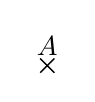
\begin{tikzpicture}[scale=0.9, baseline=-0.5ex]
\croix{2.2,0}
\node[above] at (2.2,0) {$A$};
\end{tikzpicture}\\\hline
\textbf{Droite} & Ligne droite qui n'a ni début ni fin. Par deux points distincts, il ne passe qu'\textcolor{themeColor}{une seule droite}.\newline Notation~: droite $AB$ ou droite $d$.
&
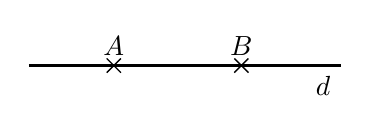
\begin{tikzpicture}[scale=0.9, baseline=-0.5ex]
\draw[thick] (0,0) -- (4.4,0) node[below left] {$d$};
\croix{1.2,0} \node[above] at (1.2,0) {$A$};
\croix{3,0} \node[above] at (3,0) {$B$};
\end{tikzpicture}\\\hline
\textbf{Demi-droite} & Portion de droite limitée par \textcolor{themeColor}{un seul point}, appelé l'origine.\newline Notation~: demi-droite $AB$, d'origine $A$ et passant par $B$.
&
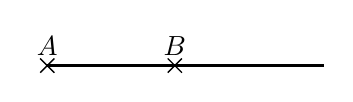
\begin{tikzpicture}[scale=0.9, baseline=-0.5ex]
\draw[thick] (0.5,0) -- (4.4,0);
\croix{0.5,0} \node[above] at (0.5,0) {$A$};
\croix{2.3,0} \node[above] at (2.3,0) {$B$};
\end{tikzpicture}\\\hline
\textbf{Segment} & Portion de droite limitée par \textcolor{themeColor}{deux points}, appelés les extrémités.\newline Notation~: segment $\overline{AB}$. Sa longueur se note $\overline{AB}$.
&
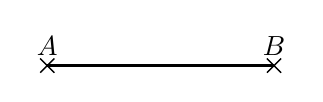
\begin{tikzpicture}[scale=0.9, baseline=-0.5ex]
\draw[thick] (0.5,0) -- (3.7,0);
\croix{0.5,0} \node[above] at (0.5,0) {$A$};
\croix{3.7,0} \node[above] at (3.7,0) {$B$};
\end{tikzpicture}\\\hline
\end{tabularx}
\def\arraystretch{1}

\vspace{6pt}
Seul le segment a une longueur : il est donc le seul à pouvoir être mesuré.

\vspace{30pt}
\begin{regle}{Définition}
Des points sont \textcolor{themeColor}{alignés} s'ils appartiennent à une même droite.
\end{regle}

\vspace{20pt}
\begin{center}
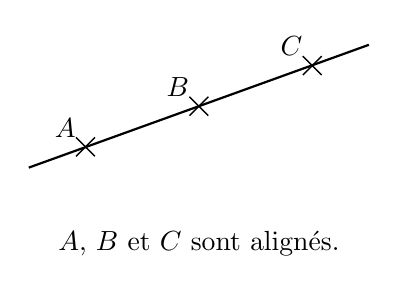
\begin{tikzpicture}[scale=1.2]
\draw[thick] (-0.3,0.2) -- (3.3,1.5);
\croix{0.3,0.42} \node[above left] at (0.3,0.42) {$A$};
\croix{1.5,0.85} \node[above left] at (1.5,0.85) {$B$};
\croix{2.7,1.28} \node[above left] at (2.7,1.28) {$C$};
\node at (1.5,-0.6) {$A$, $B$ et $C$ sont alignés.};
\end{tikzpicture}
\hspace{150pt}
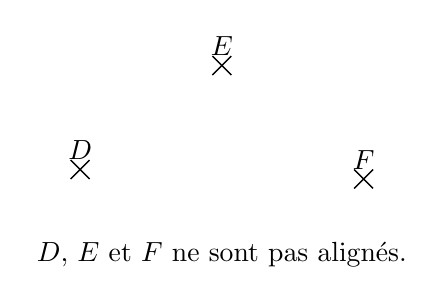
\begin{tikzpicture}[scale=1.2]
\croix{0,0.3} \node[above] at (0,0.3) {$D$};
\croix{1.5,1.4} \node[above] at (1.5,1.4) {$E$};
\croix{3,0.2} \node[above] at (3,0.2) {$F$};
\node at (1.5,-0.6) {$D$, $E$ et $F$ ne sont pas alignés.};
\end{tikzpicture}
\end{center}

\newpage
\subsection*{2. Droites sécantes, perpendiculaires et parallèles}

\def\arraystretch{1.6}
\begin{tabularx}{\linewidth}{|>{\raggedright\arraybackslash}X|>{\raggedright\arraybackslash}X|>{\raggedright\arraybackslash}X|>{\raggedright\arraybackslash}X|}
\hline
\cellcolor{themeColor!30}\textbf{Droites sécantes} & \cellcolor{themeColor!30}\textbf{Droites perpendiculaires} & \cellcolor{themeColor!30}\textbf{Droites parallèles} & \cellcolor{themeColor!30}\textbf{Droites concourantes}\\\hline
Elles ont un seul point commun, appelé \textcolor{themeColor}{point d'intersection}.
& Elles se coupent à \textcolor{themeColor}{angle droit}.\newline Notation~: $d\perp d'$
& Elles n'ont aucun point commun.\newline Notation~: $d\parallel d'$
& Elles sont au moins trois et passent par un \textcolor{themeColor}{même point}.\\\hline
\hfil
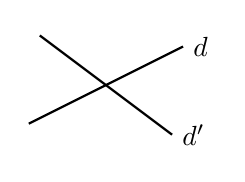
\begin{tikzpicture}[scale=0.7]
\draw[thick] (-1.4,-0.7) -- (1.4,0.7) node[right] {$d$};
\draw[thick] (-1.2,0.9) -- (1.2,-0.9) node[right] {$d'$};
\end{tikzpicture}\hfil
&
\hfil
\begin{tikzpicture}[scale=0.7]
\draw[thick] (-1.4,0) -- (1.4,0) node[right] {$d$};
\draw[thick] (0,-1) -- (0,1) node[above] {$d'$};
\draw (0.2,0) -- (0.2,0.2) -- (0,0.2);
\end{tikzpicture}\hfil
&
\hfil
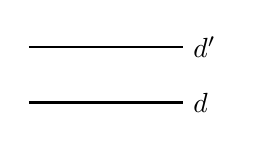
\begin{tikzpicture}[scale=0.7]
\draw[thick] (-1.4,-0.5) -- (1.4,-0.5) node[right] {$d$};
\draw[thick] (-1.4,0.5) -- (1.4,0.5) node[right] {$d'$};
\end{tikzpicture}\hfil
&
\hfil
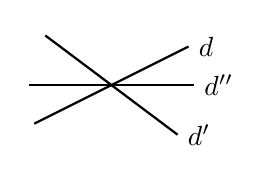
\begin{tikzpicture}[scale=0.7]
\draw[thick] (-1.4,-0.7) -- (1.4,0.7) node[right] {$d$};
\draw[thick] (-1.2,0.9) -- (1.2,-0.9) node[right] {$d'$};
\draw[thick] (-1.5,0) -- (1.5,0) node[right] {$d''$};
\end{tikzpicture}\hfil
\\\hline
\end{tabularx}
\def\arraystretch{1}


\vspace{14pt}
\begin{regle}{Propriétés}
\begin{enumerate}[leftmargin=*, itemsep=2pt, topsep=2pt]
    \item Si deux droites sont perpendiculaires à une même troisième, alors elles sont \textcolor{themeColor}{parallèles}.
    \item Si deux droites sont parallèles à une même troisième, alors elles sont \textcolor{themeColor}{parallèles entre elles}.
    \item Si deux droites sont parallèles et qu'une troisième est perpendiculaire à l'une, alors elle est \textcolor{themeColor}{perpendiculaire à l'autre}.
\end{enumerate}
\end{regle}

\vspace{6pt}
\begin{center}
\begin{tabularx}{\linewidth}{>{\centering\arraybackslash}X>{\centering\arraybackslash}X>{\centering\arraybackslash}X}
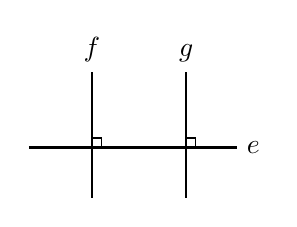
\begin{tikzpicture}[scale=0.8]
\draw[thick] (-0.3,0) -- (3,0) node[right] {$e$};
\draw[thick] (0.7,-0.8) -- (0.7,1.2) node[above] {$f$};
\draw[thick] (2.2,-0.8) -- (2.2,1.2) node[above] {$g$};
\draw (0.7,0) ++(0.15,0) -- ++(0,0.15) -- ++(-0.15,0);
\draw (2.2,0) ++(0.15,0) -- ++(0,0.15) -- ++(-0.15,0);
\end{tikzpicture}
&
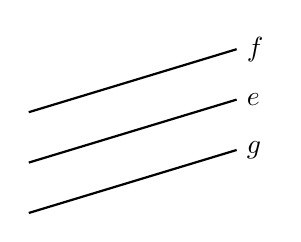
\begin{tikzpicture}[scale=0.8]
\draw[thick] (-0.3,-0.3) -- (3,0.7) node[right] {$e$};
\draw[thick] (-0.3,0.5) -- (3,1.5) node[right] {$f$};
\draw[thick] (-0.3,-1.1) -- (3,-0.1) node[right] {$g$};
\end{tikzpicture}
&
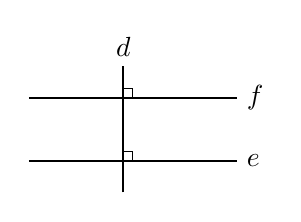
\begin{tikzpicture}[scale=0.8]
\draw[thick] (-0.3,0) -- (3,0) node[right] {$e$};
\draw[thick] (-0.3,1) -- (3,1) node[right] {$f$};
\draw[thick] (1.2,-0.5) -- (1.2,1.5) node[above] {$d$};
\draw (1.2,0) ++(0.15,0) -- ++(0,0.15) -- ++(-0.15,0);
\draw (1.2,1) ++(0.15,0) -- ++(0,0.15) -- ++(-0.15,0);
\end{tikzpicture}
\\[2pt]
{\small $f\perp e$ et $g\perp e$ donc $f\parallel g$}
&
{\small $e\parallel f$ et $g\parallel f$ donc $e\parallel g$}
&
{\small $e\parallel f$ et $d\perp e$ donc $d\perp f$}
\end{tabularx}
\end{center}

\vfill
\subsection*{3. Distances}

La \textcolor{themeColor}{distance} est toujours la longueur du \textcolor{themeColor}{plus court chemin}.

\vspace{6pt}
\def\arraystretch{1.6}
\begin{tabularx}{\linewidth}{|>{\raggedright\arraybackslash}X|>{\raggedright\arraybackslash}X|>{\raggedright\arraybackslash}X|}
\hline
\cellcolor{themeColor!30}\textbf{Entre deux points} & \cellcolor{themeColor!30}\textbf{D'un point à une droite} & \cellcolor{themeColor!30}\textbf{Entre deux droites parallèles}\\\hline
C'est la longueur du segment qui joint les deux points.
& C'est la longueur du segment perpendiculaire à la droite, qui part du point.
& C'est la longueur d'un segment perpendiculaire aux deux droites.\\\hline
\hfil
\begin{tikzpicture}[scale=0.85]
\draw[dashed, gray] (0,0) to[out=60,in=120] (3.5,0);
\draw[thick, themeColor] (0,0) -- (3.5,0);
\croix{0,0} \node[below left] at (0,0) {$A$};
\croix{3.5,0} \node[below right] at (3.5,0) {$B$};
\node[themeColor, below] at (1.75,0) {$\overline{AB}=4$ cm};
\end{tikzpicture}\hfil
&
\hfil
\begin{tikzpicture}[scale=0.85]
\draw[thick] (-0.3,0) -- (3.8,0) node[above left] {$d$};
\croix{1.5,2} \node[above] at (1.5,2) {$A$};
\croix{1.5,0} \node[below] at (1.5,0) {$H$};
\croix{2.8,0} \node[below] at (2.8,0) {$M$};
\draw[dashed, gray] (1.5,2) -- (2.8,0);
\draw[thick, themeColor] (1.5,2) -- (1.5,0);
\draw (1.5,0) ++(0.18,0) -- ++(0,0.18) -- ++(-0.18,0);
\node[themeColor, left] at (1.5,1) {$\overline{AH}$};
\end{tikzpicture}\hfil
&
\hfil
\begin{tikzpicture}[scale=0.85]
\draw[thick] (-0.3,0) -- (3.8,0) node[above left] {$d$};
\draw[thick] (-0.3,2) -- (3.8,2) node[above left] {$d'$};
\croix{1,0} \node[below] at (1,0) {$H$};
\croix{1,2} \node[above] at (1,2) {$H'$};
\draw[thick, themeColor] (1,0) -- (1,2);
\draw[dashed, gray] (2.6,0) -- (3.3,2);
\draw (1,0) ++(0.18,0) -- ++(0,0.18) -- ++(-0.18,0);
\draw (1,2) ++(0.18,0) -- ++(0,-0.18) -- ++(-0.18,0);
\node[themeColor, left] at (1,1) {$\overline{HH'}$};
\end{tikzpicture}\hfil
\\\hline
\end{tabularx}
\def\arraystretch{1}

\newpage
\subsection*{4. Le cercle}

\begin{regle}{Définition}
Un \textcolor{themeColor}{cercle} est l'ensemble des points du plan situés à la même distance d'un point appelé \textcolor{themeColor}{centre}. Cette distance est le \textcolor{themeColor}{rayon} du cercle.
\end{regle}

\vspace{8pt}
\noindent\begin{minipage}[c]{0.52\linewidth}
\textcolor{themeColor}{\textbf{Rayon}}~: segment qui joint le centre à un point du cercle (exemple~: $\overline{OM}$).\par\vspace{4pt}
\textcolor{themeColor}{\textbf{Corde}}~: segment dont les deux extrémités sont des points du cercle (exemple~: $\overline{BC}$).\par\vspace{4pt}
\textcolor{themeColor}{\textbf{Diamètre}}~: corde qui passe par le centre (exemple~: $\overline{NP}$). C'est la plus longue corde et sa longueur est le double du rayon.\par\vspace{4pt}
\textcolor{themeColor}{\textbf{Arc de cercle}}~: partie du cercle comprise entre deux points. Notation~: $\overset{\frown}{BC}$.\par\vspace{4pt}
\textcolor{themeColor}{\textbf{Disque}}~: ensemble des points situés sur le cercle et à l'intérieur de celui-ci.
\end{minipage}\hfill
\begin{minipage}[c]{0.44\linewidth}
\centering
\begin{tikzpicture}[scale=1.0]
\draw[thick] (0,0) circle (2);
\draw[thick, themeColor!60!black, line width=2pt] (230:2) arc[start angle=230, end angle=310, radius=2];
\croix{0,0} \node[below left] at (0,0) {$O$};
\croix{70:2} \node[above right] at (70:2) {$M$};
\draw[thick] (0,0) -- (70:2);
\croix{200:2} \node[left] at (200:2) {$N$};
\croix{20:2} \node[right] at (20:2) {$P$};
\draw[thick] (200:2) -- (20:2);
\croix{230:2} \node[below left] at (230:2) {$B$};
\croix{310:2} \node[below right] at (310:2) {$C$};
\draw[thick] (230:2) -- (310:2);
\node[themeColor!60!black, font=\small] at (270:2.4) {arc $BC$};
\end{tikzpicture}
\end{minipage}

\vfill
\subsection*{5. Construire des droites perpendiculaires et parallèles}

%\begin{astuce}{Perpendiculaire avec une équerre et une règle}
%\begin{enumerate}[leftmargin=*, itemsep=2pt, topsep=2pt]
%    \item Placer la règle le long de la droite $d$, puis poser l'équerre contre la règle.
%    \item Faire glisser l'équerre le long de la règle jusqu'au point $A$.
%    \item Tracer la droite qui passe par $A$ en suivant l'autre côté de l'angle droit, puis la prolonger.
%\end{enumerate}
%
%\begin{center}
%\begin{tabular}{ccc}
%\begin{tikzpicture}[scale=0.7]
%\draw[fill=gray!25] (-1.6,-0.4) rectangle (2.4,0);
%\draw[thick] (-1.6,0) -- (2.4,0) node[above left] {$d$};
%\draw[fill=themeColor!20] (-1.9,0) -- (-0.6,0) -- (-0.6,1.5) -- cycle;
%\croix{1,1.2} \node[right] at (1,1.2) {$A$};
%\node at (0.4,-0.9) {\small Étape 1};
%\end{tikzpicture}
%&
%\begin{tikzpicture}[scale=0.7]
%\draw[fill=gray!25] (-1.6,-0.4) rectangle (2.4,0);
%\draw[thick] (-1.6,0) -- (2.4,0) node[above left] {$d$};
%\draw[fill=themeColor!20] (-0.3,0) -- (1,0) -- (1,1.5) -- cycle;
%\croix{1,1.2} \node[right] at (1,1.2) {$A$};
%\node at (0.4,-0.9) {\small Étape 2};
%\end{tikzpicture}
%&
%\begin{tikzpicture}[scale=0.7]
%\draw[fill=gray!25] (-1.6,-0.4) rectangle (2.4,0);
%\draw[thick] (-1.6,0) -- (2.4,0) node[above left] {$d$};
%\draw[thick, themeColor] (1,-0.2) -- (1,1.9);
%\draw (1,0) ++(0.2,0) -- ++(0,0.2) -- ++(-0.2,0);
%\croix{1,1.2} \node[right] at (1,1.2) {$A$};
%\node at (0.4,-0.9) {\small Étape 3};
%\end{tikzpicture}
%\end{tabular}
%\end{center}
%\end{astuce}
%
%\vspace{10pt}
%\begin{astuce}{Parallèle avec une équerre et une règle}
%\begin{enumerate}[leftmargin=*, itemsep=2pt, topsep=2pt]
%    \item Poser un côté de l'angle droit de l'équerre sur la droite $d$, puis placer la règle contre l'autre côté de l'angle droit.
%    \item Faire glisser l'équerre le long de la règle jusqu'au point $A$.
%    \item Tracer la droite qui passe par $A$ en suivant le côté de l'équerre qui était sur $d$.
%\end{enumerate}
%
%\begin{center}
%\begin{tabular}{ccc}
%\begin{tikzpicture}[scale=0.7]
%\draw[thick] (-1.8,0) -- (0,0) node[pos=0, left] {$d$};
%\draw[fill=gray!25] (0,-0.3) rectangle (0.4,3.2);
%\draw[fill=themeColor!20] (-1.3,0) -- (0,0) -- (0,1.2) -- cycle;
%\croix{-0.8,1.8} \node[left] at (-0.8,1.8) {$A$};
%\node at (-0.6,-0.8) {\small Étape 1};
%\end{tikzpicture}
%&
%\begin{tikzpicture}[scale=0.7]
%\draw[thick] (-1.8,0) -- (0,0) node[pos=0, left] {$d$};
%\draw[fill=gray!25] (0,-0.3) rectangle (0.4,3.2);
%\draw[fill=themeColor!20] (-1.3,1.8) -- (0,1.8) -- (0,3) -- cycle;
%\croix{-0.8,1.8} \node[below left] at (-0.8,1.8) {$A$};
%\node at (-0.6,-0.8) {\small Étape 2};
%\end{tikzpicture}
%&
%\begin{tikzpicture}[scale=0.7]
%\draw[thick] (-1.8,0) -- (0,0) node[pos=0, left] {$d$};
%\draw[fill=gray!25] (0,-0.3) rectangle (0.4,3.2);
%\draw[thick, themeColor] (-1.8,1.8) -- (0,1.8);
%\croix{-0.8,1.8} \node[above] at (-0.8,1.8) {$A$};
%\node at (-0.6,-0.8) {\small Étape 3};
%\end{tikzpicture}
%\end{tabular}
%\end{center}
%\end{astuce}

\begin{astuce}{Perpendiculaire avec un compas et une règle}
\begin{enumerate}[leftmargin=*, itemsep=2pt, topsep=2pt]
    \item Avec le compas centré en $A$, tracer un arc de cercle qui coupe la droite $d$ en deux points $P$ et $Q$.
    \item Avec le compas centré en $P$, puis en $Q$, tracer deux arcs de cercle de même rayon qui se coupent en un point $B$.
    \item Tracer la droite $AB$ : elle est perpendiculaire à $d$ et passe par $A$.
\end{enumerate}
\end{astuce}

\vspace{10pt}
\begin{center}
\begin{tikzpicture}[scale=1]
\draw[thick] (-3.2,0) -- (3.2,0) node[above] {$d$};
\croix{0,2} \node[above right] at (0,2) {$A$};
\draw[gray] ([shift=(-143:2.8)]0,2) arc[start angle=-143, end angle=-37, radius=2.8];
\croix{-1.96,0} \node[above left] at (-1.96,0) {$P$};
\croix{1.96,0} \node[above right] at (1.96,0) {$Q$};
\draw[gray] ([shift=(-60:2.5)]-1.96,0) arc[start angle=-60, end angle=-15, radius=2.5];
\draw[gray] ([shift=(195:2.5)]1.96,0) arc[start angle=195, end angle=240, radius=2.5];
\croix{0,-1.55} \node[below right] at (0,-1.55) {$B$};
\draw[thick, themeColor] (0,2.5) -- (0,-2);
\draw (0,0) ++(0.2,0) -- ++(0,0.2) -- ++(-0.2,0);
\end{tikzpicture}
\end{center}

\newpage
\begin{astuce}{Parallèle avec un compas et une règle}
\begin{enumerate}[leftmargin=*, itemsep=2pt, topsep=2pt]
    \item Choisir un point $B$ sur la droite $d$ et ouvrir le compas de la longueur $\overline{BA}$.
    \item Avec le compas centré en $B$, tracer un arc de cercle qui coupe $d$ en un point $C$.
    \item Sans changer l'ouverture, tracer un arc de cercle centré en $A$, puis un autre centré en $C$ : ils se coupent en un point $D$.
    \item Tracer la droite $AD$ : elle est parallèle à $d$ (le quadrilatère $ABCD$ est un losange).
\end{enumerate}
\end{astuce}

\vspace{6pt}
\begin{center}
\begin{tikzpicture}[scale=1]
\draw[thick] (-1.2,0) -- (3,0) node[above] {$d$};
\croix{0,0} \node[below] at (0,0) {$B$};
\croix{1.879,0} \node[below] at (1.879,0) {$C$};
\croix{-0.8,1.7} \node[above left] at (-0.8,1.7) {$A$};
\croix{1.079,1.7} \node[above right] at (1.079,1.7) {$D$};
\draw[gray] ([shift=(115.2:1.879)]0,0) arc[start angle=115.2, end angle=0, radius=1.879];
\draw[gray] ([shift=(-30:1.879)]-0.8,1.7) arc[start angle=-30, end angle=30, radius=1.879];
\draw[gray] ([shift=(85:1.879)]1.879,0) arc[start angle=85, end angle=145, radius=1.879];
\draw[thick, themeColor] (-1.4,1.7) -- (2.3,1.7);
\end{tikzpicture}
\end{center}
\vspace{-6pt}

\vfill
\subsection*{6. Les angles}

\begin{regle}{Définition}
Un \textcolor{themeColor}{angle} est une portion de plan limitée par deux demi-droites de même origine. Cette origine est le \textcolor{themeColor}{sommet} de l'angle et les demi-droites sont ses \textcolor{themeColor}{côtés}.
\end{regle}

\begin{center}
\begin{tikzpicture}[scale=0.8]
\draw[thick] (0,0) -- (3.2,0) node[right] {$B$};
\draw[thick] (0,0) -- (35:3.2) node[above right] {$A$};
\draw[themeColor, thick] (0.9,0) arc[start angle=0, end angle=35, radius=0.9];
\node[themeColor] at (17:1.25) {$\alpha$};
\croix{0,0} \node[below left] at (0,0) {$O$};
\node[font=\small, gray!60!black] at (2,-0.4) {côté};
\node[font=\small, gray!60!black] at (1.2,1.4) {côté};
\node[font=\small, gray!60!black, anchor=east] at (-0.6,-0.45) {sommet};
\end{tikzpicture}
\end{center}

\begin{astuce}{Notation}
Un angle se note avec trois lettres, le \textcolor{themeColor}{sommet} au milieu~: $\widehat{BOA}$.\\[2pt]
On peut aussi le désigner par une lettre grecque~: $\alpha$, $\beta$, $\gamma$, \ldots\\[2pt]
L'unité usuelle de mesure des angles est le \textcolor{themeColor}{degré}, noté $^\circ$.
\end{astuce}

\vfill
\subsection*{7. Les types d'angles}

\begin{center}
\def\arraystretch{1}
\setlength{\tabcolsep}{2pt}
\small
\begin{tabularx}{\linewidth}{*{7}{>{\centering\arraybackslash}X}}
\angfig{0} & \angfig{50} & \angfig{90} & \angfig{130} & \angfig{180} & \angfig{240} & \angfig{360}\\
\textbf{Nul} & \textbf{Aigu} & \textbf{Droit} & \textbf{Obtus} & \textbf{Plat} & \textbf{Rentrant} & \textbf{Plein}\\
$0^\circ$ & $0^\circ<\alpha<90^\circ$ & $90^\circ$ & $90^\circ<\alpha<180^\circ$ & $180^\circ$ & $180^\circ<\alpha<360^\circ$ & $360^\circ$
\end{tabularx}
\end{center}

\newpage
%\vfill
%\subsection*{8. Mesurer et construire un angle}
%
%\begin{astuce}{Mesurer un angle avec un rapporteur}
%\begin{enumerate}[leftmargin=*, itemsep=2pt, topsep=2pt]
%    \item Estimer à vue d'oeil si l'angle est aigu ou obtus.
%    \item Placer le centre du rapporteur sur le sommet de l'angle.
%    \item Faire coïncider un côté de l'angle avec le $0^\circ$ d'une des graduations.
%    \item Lire la mesure sur cette graduation.
%    \item Vérifier que la valeur est cohérente avec l'estimation de l'étape 1.
%\end{enumerate}
%
%\vspace{6pt}
%\begin{center}
%\begin{tikzpicture}[scale=1.15]
%\rapporteur
%\draw[thick] (0,0) -- (2.4,0) node[right] {$B$};
%\draw[thick] (0,0) -- (35:2.4) node[above right] {$A$};
%\draw[themeColor, very thick] (35:1.1) -- (35:1.4);
%\croix{0,0}
%\node[above left] at (0,0) {$O$};
%\node[themeColor!70!black, font=\small] at (17:1.85) {$35^\circ$};
%\end{tikzpicture}
%\end{center}
%\end{astuce}
%
%\vspace{10pt}
%\begin{astuce}{Construire un angle avec un rapporteur}
%\begin{enumerate}[leftmargin=*, itemsep=2pt, topsep=2pt]
%    \item Tracer une demi-droite d'origine $O$.
%    \item Placer le centre du rapporteur sur $O$ et le $0^\circ$ sur la demi-droite.
%    \item Marquer un point à la mesure voulue, sur la bonne graduation.
%    \item Tracer la demi-droite d'origine $O$ qui passe par ce point.
%\end{enumerate}
%
%\vspace{6pt}
%\begin{center}
%\begin{tikzpicture}[scale=1.15]
%\rapporteur
%\draw[thick] (0,0) -- (2.4,0) node[right] {$B$};
%\croix{50:1.55}
%\node[above] at (50:1.6) {$P$};
%\draw[themeColor, thick] (0,0) -- (50:2.4);
%\croix{0,0}
%\node[above left] at (0,0) {$O$};
%\node[themeColor!70!black, font=\small] at (25:1.85) {$50^\circ$};
%\end{tikzpicture}
%\end{center}
%\end{astuce}
%
%\vspace{10pt}
%\begin{astuce}{Estimer un angle à vue d'oeil}
%Comparer l'angle à des repères~: un angle droit ($90^\circ$) est le coin d'une feuille, un angle plat ($180^\circ$) forme une ligne droite, et un angle de $45^\circ$ est la moitié d'un angle droit.
%\end{astuce}

\providecommand{\croix}[1]{\draw[line width=0.5pt] (#1) ++(-0.1,-0.1) -- ++(0.2,0.2) (#1) ++(-0.1,0.1) -- ++(0.2,-0.2);}
% codage : un trait / deux traits au milieu d'un côté, flèche de parallélisme, angle droit
\providecommand{\tA}{node[midway, sloped, inner sep=0pt]{\tiny$\mid$}}
\providecommand{\tB}{node[midway, sloped, inner sep=0pt]{\tiny$\mid\mid$}}
\providecommand{\fl}{node[pos=0.72, sloped, inner sep=0pt]{\tiny$>$}}
\providecommand{\puceT}[1]{\hangindent=1em\hangafter=1\noindent\textbullet\,#1\par}
\providecommand{\sqm}[4]{\draw[line width=0.4pt] ({#1+#3*0.18},{#2}) -- ({#1+#3*0.18},{#2+#4*0.18}) -- ({#1},{#2+#4*0.18});}

\subsection*{9. Axe et centre de symétrie}

\begin{regle}{Définitions}
Un \textcolor{themeColor}{axe de symétrie} est une droite qui partage une figure en deux parties qui se superposent exactement lorsqu'on plie la figure le long de cette droite.\\[2pt]
Un \textcolor{themeColor}{centre de symétrie} est un point autour duquel on peut faire faire un demi-tour à la figure pour qu'elle se superpose exactement à elle-même.
\end{regle}

\vspace{6pt}
\begin{center}
\begin{tikzpicture}[scale=0.9]
\draw[thick] (0,0) rectangle (3,1.6);
\draw[themeColor, dashed, thick] (1.5,-0.3) -- (1.5,1.9);
\draw[themeColor, dashed, thick] (-0.3,0.8) -- (3.3,0.8);
\croix{1.5,0.8}
\node[font=\small] at (1.5,-0.7) {Un rectangle a deux axes de symétrie};
\node[font=\small] at (1.5,-1.15) {et un centre de symétrie.};
\end{tikzpicture}
\end{center}

\vfill
\subsection*{10. Les triangles}

\begin{regle}{Définition}
Un \textcolor{themeColor}{triangle} est un \textcolor{themeColor}{polygone} qui a trois côtés. Il a aussi trois angles et trois sommets.
\end{regle}

\vspace{10pt}
\begin{regle}{Propriété}
La somme des mesures des angles d'un triangle est égale à \textcolor{themeColor}{$180^\circ$}.
\end{regle}


\def\arraystretch{1.2}
\begin{tabularx}{\linewidth}{|>{\centering\arraybackslash}m{2.2cm}|>{\centering\arraybackslash}m{3cm}|>{\raggedright\arraybackslash}X|>{\raggedright\arraybackslash}X|>{\raggedright\arraybackslash}X|}
\hline
\cellcolor{themeColor!30}\textbf{Nom} & \cellcolor{themeColor!30}\textbf{Figure} & \cellcolor{themeColor!30}\textbf{Côtés} & \cellcolor{themeColor!30}\textbf{Angles} & \cellcolor{themeColor!30}\textbf{Symétries}\\\hline
\textbf{Triangle quelconque}
&
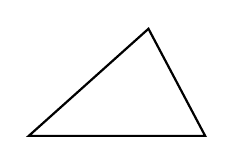
\begin{tikzpicture}[scale=0.8]
\draw[thick] (0,0) -- (2.8,0) -- (1.9,1.7) -- cycle;
\end{tikzpicture}
& &  & \\\hline
\textbf{Triangle isocèle}
&
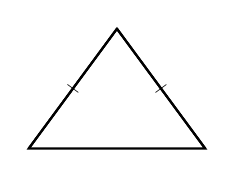
\begin{tikzpicture}[scale=0.8]
\draw[thick] (0,0) -- (2.8,0) -- (1.4,1.9) -- cycle;
\draw[thick] (0,0) -- (1.4,1.9) \tA;
\draw[thick] (2.8,0) -- (1.4,1.9) \tA;
\end{tikzpicture}
& Au moins deux côtés isométriques. & Au moins deux angles isométriques. & Au moins un axe de symétrie.\\\hline
\textbf{Triangle équilatéral}
&
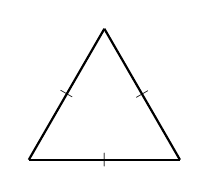
\begin{tikzpicture}[scale=0.8]
\draw[thick] (0,0) -- (2.4,0) \tA;
\draw[thick] (2.4,0) -- (1.2,2.08) \tA;
\draw[thick] (1.2,2.08) -- (0,0) \tA;
\end{tikzpicture}
& Trois côtés isométriques. & Trois angles de $60^\circ$. & Trois axes de symétrie.\\\hline
\textbf{Triangle rectangle}
&
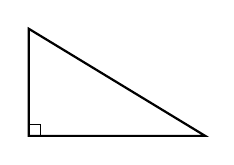
\begin{tikzpicture}[scale=0.8]
\draw[thick] (0,0) -- (2.8,0) -- (0,1.7) -- cycle;
\sqm{0}{0}{1}{1}
\end{tikzpicture}
& Deux côtés perpendiculaires. & Un angle droit. & \\\hline
\textbf{Triangle rectangle isocèle}
&
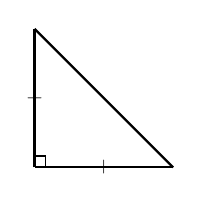
\begin{tikzpicture}[scale=0.8]
\draw[thick] (0,0) -- (2.2,0) \tA;
\draw[thick] (0,0) -- (0,2.2) \tA;
\draw[thick] (2.2,0) -- (0,2.2);
\sqm{0}{0}{1}{1}
\end{tikzpicture}
& Deux côtés isométriques et perpendiculaires. & Un angle droit et deux angles de $45^\circ$. & Un axe de symétrie.\\\hline
\end{tabularx}
\def\arraystretch{1}

\newpage
\subsection*{11. Les quadrilatères}

\begin{regle}{Définition}
Un \textcolor{themeColor}{quadrilatère} est un \textcolor{themeColor}{polygone} qui a quatre côtés. Il a aussi quatre angles et quatre sommets.
\end{regle}

\begin{center}
\begin{tikzpicture}[scale=0.7]
\coordinate (A) at (0,0);
\coordinate (B) at (3,0.2);
\coordinate (C) at (3.4,1.9);
\coordinate (D) at (0.5,1.6);
\draw[thick] (A) -- (B) -- (C) -- (D) -- cycle;
\draw[themeColor, dashed, thick] (A) -- (C);
\draw[themeColor, dashed, thick] (B) -- (D);
\node[below left] at (A) {$A$};
\node[below right] at (B) {$B$};
\node[above right] at (C) {$C$};
\node[above left] at (D) {$D$};
\end{tikzpicture}
\end{center}

\begin{itemize}[leftmargin=*, itemsep=2pt, topsep=2pt, label=$\triangleright$]
    \item Les côtés $\overline{AB}$ et $\overline{DC}$, ainsi que $\overline{AD}$ et $\overline{BC}$, sont des \textcolor{themeColor}{côtés opposés}.
    \item Les côtés $\overline{AB}$ et $\overline{BC}$ sont des \textcolor{themeColor}{côtés consécutifs}.
    \item Les angles $\widehat{BAD}$ et $\widehat{DCB}$, ainsi que $\widehat{CBA}$ et $\widehat{ADC}$, sont des \textcolor{themeColor}{angles opposés}.
    \item Une \textcolor{themeColor}{diagonale} est un segment qui relie deux sommets opposés ($\overline{AC}$ et $\overline{BD}$).
\end{itemize}

\begin{regle}{Propriété}
La somme des mesures des angles d'un quadrilatère est égale à \textcolor{themeColor}{$360^\circ$}.
\end{regle}

\vfill
\subsection*{12. Les quadrilatères particuliers}

\def\arraystretch{1.7}
\small
\setlength{\tabcolsep}{4pt}
\begin{tabularx}{\linewidth}{|>{\centering\arraybackslash}m{2.2cm}|>{\centering\arraybackslash}m{2.5cm}|>{\raggedright\arraybackslash}X|>{\raggedright\arraybackslash}X|>{\raggedright\arraybackslash}X|>{\raggedright\arraybackslash}X|}
\hline
\cellcolor{themeColor!30}\textbf{Nom} & \cellcolor{themeColor!30}\textbf{Figure} & \cellcolor{themeColor!30}\textbf{Côtés} & \cellcolor{themeColor!30}\textbf{Angles} & \cellcolor{themeColor!30}\textbf{Symétries} & \cellcolor{themeColor!30}\textbf{Diagonales}\\\hline
\textbf{Trapèze quelcon\-que}
&
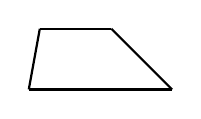
\begin{tikzpicture}[scale=0.7]
\draw[thick] (0,0) -- (2.6,0) ;
\draw[thick] (2.6,0) -- (1.5,1.1);
\draw[thick] (0.2,1.1) -- (1.5,1.1) ;
\draw[thick] (0,0) -- (0.2,1.1);
\end{tikzpicture}
& Au moins une paire de côtés parallèles. &  &  & \\\hline
\textbf{Trapèze rectangle}
&
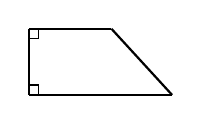
\begin{tikzpicture}[scale=0.7]
\draw[thick] (0,0) -- (2.6,0) ;
\draw[thick] (2.6,0) -- (1.5,1.2);
\draw[thick] (0,1.2) -- (1.5,1.2);
\draw[thick] (0,0) -- (0,1.2);
\sqm{0}{0}{1}{1}
\sqm{0}{1.2}{1}{-1}
\end{tikzpicture}
& Au moins une paire de côtés parallèles et un côté perpendiculaire aux côtés parallèles. & Deux angles droits. & Aucun axe de symétrie. & Aucune propriété particulière.\\\hline
\textbf{Trapèze isocèle}
&
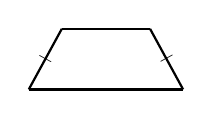
\begin{tikzpicture}[scale=0.7]
\draw[thick] (0,0) -- (2.8,0) ;
\draw[thick] (2.8,0) -- (2.2,1.1) \tA;
\draw[thick] (0.6,1.1) -- (2.2,1.1) ;
\draw[thick] (0,0) -- (0.6,1.1) \tA;
\end{tikzpicture}
& Au moins une paire de côtés parallèles et les deux autres côtés isométriques. & Deux paires d'angles isométriques. & Un axe de symétrie. & Diagonales isométriques.\\\hline
\end{tabularx}
\normalsize

\newpage
\small
\setlength{\tabcolsep}{4pt}
\begin{tabularx}{\linewidth}{|>{\centering\arraybackslash}m{2.2cm}|>{\centering\arraybackslash}m{2.5cm}|>{\raggedright\arraybackslash}X|>{\raggedright\arraybackslash}X|>{\raggedright\arraybackslash}X|>{\raggedright\arraybackslash}X|}
\hline
\cellcolor{themeColor!30}\textbf{Nom} & \cellcolor{themeColor!30}\textbf{Figure} & \cellcolor{themeColor!30}\textbf{Côtés} & \cellcolor{themeColor!30}\textbf{Angles} & \cellcolor{themeColor!30}\textbf{Symétries} & \cellcolor{themeColor!30}\textbf{Diagonales}\\\hline
\textbf{Parallélo\-gramme}
&
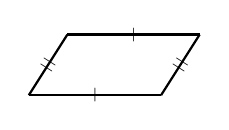
\begin{tikzpicture}[scale=0.7]
\draw[thick] (0,0) -- (2.4,0) \tA ;
\draw[thick] (2.4,0) -- (3.1,1.1) \tB;
\draw[thick] (0.7,1.1) -- (3.1,1.1) \tA ;
\draw[thick] (0,0) -- (0.7,1.1) \tB;
\end{tikzpicture}
& Deux paires de côtés parallèles et isométriques. & Angles opposés isométriques. & Un centre de symétrie. & Elles se coupent en leur milieu.\\\hline
\textbf{Rectangle}
&
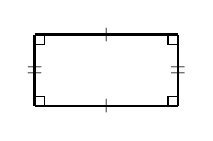
\begin{tikzpicture}[scale=0.7]
\draw[thick] (0,0) -- (2.6,0) \tA;
\draw[thick] (2.6,0) -- (2.6,1.3) \tB;
\draw[thick] (0,1.3) -- (2.6,1.3) \tA;
\draw[thick] (0,0) -- (0,1.3) \tB;
\sqm{0}{0}{1}{1}
\sqm{2.6}{0}{-1}{1}
\sqm{2.6}{1.3}{-1}{-1}
\sqm{0}{1.3}{1}{-1}
\end{tikzpicture}
& Côtés opposés parallèles et isométriques. & Quatre angles droits. & Un centre de symétrie et deux axes de symétrie. & Isométriques. Elles se coupent en leur milieu.\\\hline
\textbf{Losange}
&
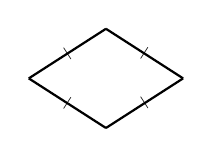
\begin{tikzpicture}[scale=0.7]
\draw[thick] (1.4,0) -- (2.8,0.9) \tA;
\draw[thick] (2.8,0.9) -- (1.4,1.8) \tA;
\draw[thick] (1.4,1.8) -- (0,0.9) \tA;
\draw[thick] (0,0.9) -- (1.4,0) \tA;
\end{tikzpicture}
& Quatre côtés isométriques. Côtés opposés parallèles. & Angles opposés isométriques. & Un centre de symétrie et deux axes de symétrie (les diagonales). & Perpendiculaires. Elles se coupent en leur milieu.\\\hline
\textbf{Carré}
&
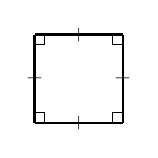
\begin{tikzpicture}[scale=0.7]
\draw[thick] (0,0) -- (1.6,0) \tA;
\draw[thick] (1.6,0) -- (1.6,1.6) \tA;
\draw[thick] (0,1.6) -- (1.6,1.6) \tA;
\draw[thick] (0,0) -- (0,1.6) \tA;
\sqm{0}{0}{1}{1}
\sqm{1.6}{0}{-1}{1}
\sqm{1.6}{1.6}{-1}{-1}
\sqm{0}{1.6}{1}{-1}
\end{tikzpicture}
& Quatre côtés isométriques. Côtés opposés parallèles. & Quatre angles droits. & Un centre de symétrie et quatre axes de symétrie. & Isométriques et perpendiculaires. Elles se coupent en leur milieu.\\\hline
\textbf{Cerf-volant}
&
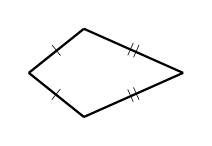
\begin{tikzpicture}[scale=0.7]
\draw[thick] (0,0.9) -- (1.0,1.7) \tA;
\draw[thick] (1.0,1.7) -- (2.8,0.9) \tB;
\draw[thick] (2.8,0.9) -- (1.0,0.1) \tB;
\draw[thick] (1.0,0.1) -- (0,0.9) \tA;
\end{tikzpicture}
& Deux paires de côtés consécutifs isométriques. Figure convexe. & Au moins deux angles opposés isométriques. & Un axe de symétrie (une diagonale). & Perpendiculaires. L'une coupe l'autre en son milieu.\\\hline
\textbf{Fer de lance}
&
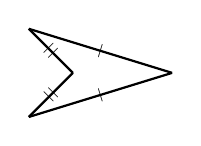
\begin{tikzpicture}[scale=0.7]
\draw[thick] (2.8,0.9) -- (0.2,1.7) \tA;
\draw[thick] (0.2,1.7) -- (1.0,0.9) \tB;
\draw[thick] (1.0,0.9) -- (0.2,0.1) \tB;
\draw[thick] (0.2,0.1) -- (2.8,0.9) \tA;
\end{tikzpicture}
& Deux paires de côtés consécutifs isométriques. Figure non convexe. & Au moins deux angles opposés isométriques. & Un axe de symétrie (une diagonale). & Perpendiculaires. L'une coupe l'autre en son milieu.\\\hline
\end{tabularx}
\normalsize
\def\arraystretch{1}

\providecommand{\just}[2]{\noindent\begin{tabular}{@{}>{\raggedright\arraybackslash}p{7.3cm}!{\color{themeColor}\vrule width 0.8pt}@{\hspace{8pt}}>{\raggedright\arraybackslash}p{6.4cm}@{}}#1&#2\end{tabular}}

\newpage
\subsection*{13. Calculs d'angles}

Pour calculer un angle, on utilise les propriétés des figures. Chaque calcul doit être \textcolor{themeColor}{justifié} : à droite du calcul, on indique la propriété qui permet de l'écrire.

\vspace{6pt}
\begin{regle}{Marche à suivre}
\begin{enumerate}[leftmargin=*, itemsep=2pt, topsep=2pt, label=\textcolor{themeColor}{\textbf{\arabic*.}}]
    \item Écrire le \textbf{nom de l'angle} qui nous intéresse (ou une lettre grecque : $\alpha$, $\beta$, $\delta$\ldots).
    \item Écrire le \textbf{calcul}, ligne par ligne.
    \item Donner la \textbf{réponse avec l'unité} ($^\circ$).
    \item Écrire la \textbf{justification} à droite de chaque ligne, après un trait vertical.
\end{enumerate}
\end{regle}

\vspace{10pt}
\noindent\textbf{Exemple 1}\quad Dans le triangle $ABC$ isocèle en $A$, $\widehat{CBA}=35^\circ$. Calculer $\widehat{BAC}$.

\vspace{6pt}
\begin{center}
\begin{tikzpicture}[scale=1.1]
\coordinate (A) at (2.6,1.8);
\coordinate (B) at (0,0);
\coordinate (C) at (5.2,0);
\draw[thick] (B) -- (C);
\draw[thick] (A) -- (B) \tA;
\draw[thick] (A) -- (C) \tA;
\node[above] at (A) {$A$};
\node[below left] at (B) {$B$};
\node[below right] at (C) {$C$};
\draw[themeColor] (0.8,0) arc[start angle=0, end angle=35.8, radius=0.8];
\node[themeColor!70!black, font=\small] at (1.15,0.25) {$35^\circ$};
\end{tikzpicture}
\end{center}

\vspace{4pt}
\renewcommand{\arraystretch}{1.6}
\just{$\widehat{CBA}=\widehat{ACB}=35^\circ$}{$\triangle_{ABC}$ isocèle en $A$}\\
\just{$\widehat{BAC}=180-2\cdot 35=110^\circ$}{somme angles $\triangle_{ABC}$}
\renewcommand{\arraystretch}{1}

\vspace{14pt}
\noindent\textbf{Exemple 2}\quad Dans le parallélogramme $ABCD$, $\widehat{BAD}=70^\circ$. Calculer $\widehat{CBA}$.

\vspace{6pt}
\begin{center}
\begin{tikzpicture}[scale=1.1]
\coordinate (A) at (0,0);
\coordinate (B) at (3.2,0);
\coordinate (D) at (0.62,1.69);
\coordinate (C) at (3.82,1.69);
\draw[thick] (A) -- (B) \tA;
\draw[thick] (B) -- (C) \tB;
\draw[thick] (D) -- (C) \tA;
\draw[thick] (A) -- (D) \tB;
\node[below left] at (A) {$A$};
\node[below right] at (B) {$B$};
\node[above right] at (C) {$C$};
\node[above left] at (D) {$D$};
\draw[themeColor] (0.7,0) arc[start angle=0, end angle=70, radius=0.7];
\node[themeColor!70!black, font=\small] at (1.0,0.4) {$70^\circ$};
\end{tikzpicture}
\end{center}

\vspace{4pt}
\renewcommand{\arraystretch}{1.6}
\just{$\widehat{DCB}=\widehat{BAD}=70^\circ$}{angles opposés du parallélogramme $ABCD$ isométriques}\\
\just{$\widehat{CBA}+\widehat{ADC}=360-2\cdot 70=220^\circ$}{somme angles $\square_{ABCD}$}\\
\just{$\widehat{CBA}=\widehat{ADC}=220:2=110^\circ$}{angles opposés du parallélogramme $ABCD$ isométriques}
\renewcommand{\arraystretch}{1}

\vspace{14pt}
\subsection*{14. Exemples de justifications}

\def\arraystretch{1.8}\setlength{\extrarowheight}{3pt}
\small
\begin{tabularx}{\linewidth}{|>{\raggedright\arraybackslash}X|>{\raggedright\arraybackslash}m{6.7cm}|}
\hline
\cellcolor{themeColor!30}\textbf{Propriété utilisée} & \cellcolor{themeColor!30}\textbf{Justification à écrire}\\\hline
La somme des mesures des angles d'un triangle vaut $180^\circ$. & somme angles $\triangle_{ABC}$\\\hline
La somme des mesures des angles d'un quadrilatère vaut $360^\circ$. & somme angles $\square_{MNOP}$\\\hline
Un triangle isocèle a deux angles isométriques. & $\triangle_{IJK}$ isocèle en $J$\\\hline
Un triangle équilatéral a trois angles de $60^\circ$. & $\triangle_{QRS}$ équilatéral\\\hline
Un triangle rectangle a un angle droit. & $\triangle_{DEF}$ rectangle en $E$\\\hline
Un trapèze isocèle a deux paires d'angles isométriques. & trapèze $ABCD$ isocèle\\\hline
Un parallélogramme a ses angles opposés isométriques. & angles opposés du parallélogramme $STUV$ isométriques\\\hline
Un rectangle et un carré ont quatre angles droits. & rectangle $EFGH$\\\hline
Les diagonales d'un losange sont perpendiculaires. & diagonales du losange $DEFG$ perpendiculaires\\\hline
\end{tabularx}
\normalsize
\def\arraystretch{1}\setlength{\extrarowheight}{0pt}

\vfill
\subsection*{15. Croquis et codage}

\begin{regle}{Définition}
Un \textcolor{themeColor}{croquis} est un dessin fait à main levée, sans instruments. Il ne respecte pas les mesures, mais il montre la \textcolor{themeColor}{forme} de la figure et ses \textcolor{themeColor}{propriétés}. Pour les indiquer, on utilise le \textcolor{themeColor}{codage}.
\end{regle}

\vspace{8pt}
\def\arraystretch{1.5}\setlength{\extrarowheight}{3pt}
\begin{tabularx}{\linewidth}{|>{\centering\arraybackslash}m{4.2cm}|>{\raggedright\arraybackslash}X|}
\hline
\cellcolor{themeColor!30}\textbf{Codage} & \cellcolor{themeColor!30}\textbf{Signification}\\\hline
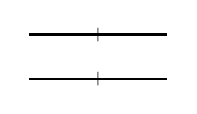
\begin{tikzpicture}[scale=0.8]
\draw[thick] (0,0) -- (2.2,0) \tA;
\draw[thick] (0,0.7) -- (2.2,0.7) \tA;
\end{tikzpicture}
& Les segments qui portent le même nombre de traits sont isométriques (ils ont la même longueur).\\\hline
\begin{tikzpicture}[scale=0.8]
\draw[thick] (0,0) -- (2,0);
\draw[thick] (0,0) -- (0,1.2);
\sqm{0}{0}{1}{1}
\end{tikzpicture}
& Un petit carré indique un angle droit ($90^\circ$).\\\hline
\begin{tikzpicture}[scale=0.8]
\draw[thick] (0,0) -- (1.8,0);
\draw[thick] (0,0) -- (1.3,1.1);
\draw[themeColor] (0.6,0) arc[start angle=0, end angle=40, radius=0.6];
\node[themeColor!70!black, font=\small] at (0.95,0.2) {$40^\circ$};
\end{tikzpicture}
& On écrit les mesures connues (longueurs et angles) à côté du segment ou de l'angle concerné.\\\hline
\end{tabularx}
\def\arraystretch{1}\setlength{\extrarowheight}{0pt}

\newpage
\begin{regle}{Marche à suivre}
\begin{enumerate}[leftmargin=*, itemsep=2pt, topsep=2pt, label=\textcolor{themeColor}{\textbf{\arabic*.}}]
    \item Lire l'énoncé et repérer la figure à dessiner.
    \item Dessiner à main levée une figure qui lui \textbf{ressemble}:
    \item[]un angle droit doit avoir l'air droit, des côtés isométriques la même longueur.
    \item \textbf{Nommer} les sommets.
    \item \textbf{Coder} les propriétés de la figure.
    \item \textbf{Noter} les mesures données par l'énoncé.
\end{enumerate}
\end{regle}

\vspace{10pt}
\noindent\begin{minipage}[t]{0.48\linewidth}
\textbf{Exemple 1}\\[3pt]
Le rectangle $ABCD$ tel que $\overline{AB}=6$ cm et $\overline{BC}=3$ cm.

\vspace{4pt}
\centering
\begin{tikzpicture}[scale=0.75]
\coordinate (A) at (0,0);
\coordinate (B) at (4.2,0.05);
\coordinate (C) at (4.15,2.1);
\coordinate (D) at (-0.05,2.05);
\draw[thick] (A) -- (B) \tA;
\draw[thick] (B) -- (C) \tB;
\draw[thick] (D) -- (C) \tA;
\draw[thick] (A) -- (D) \tB;
\sqm{0}{0}{1}{1}
\sqm{4.2}{0.05}{-1}{1}
\sqm{4.15}{2.1}{-1}{-1}
\sqm{-0.05}{2.05}{1}{-1}
\node[below left] at (A) {$A$};
\node[below right] at (B) {$B$};
\node[above right] at (C) {$C$};
\node[above left] at (D) {$D$};
\node[below, font=\small] at (2.1,0) {6 cm};
\node[right, font=\small] at (4.2,1.05) {3 cm};
\end{tikzpicture}
\end{minipage}\hfill
\begin{minipage}[t]{0.48\linewidth}
\textbf{Exemple 2}\\[3pt]
Le triangle $ABC$ isocèle en $A$ tel que $\overline{BC}=5$ cm et $\widehat{ABC}=40^\circ$.

\vspace{4pt}
\centering
\begin{tikzpicture}[scale=0.75]
\coordinate (A) at (2.1,1.8);
\coordinate (B) at (0,0);
\coordinate (C) at (4.2,0);
\draw[thick] (B) -- (C);
\draw[thick] (A) -- (B) \tA;
\draw[thick] (A) -- (C) \tA;
\node[above] at (A) {$A$};
\node[below left] at (B) {$B$};
\node[below right] at (C) {$C$};
\node[below, font=\small] at (2.1,0) {5 cm};
\draw[themeColor] (0.8,0) arc[start angle=0, end angle=40, radius=0.8];
\node[themeColor!70!black, font=\small] at (1.2,0.3) {$40^\circ$};
\end{tikzpicture}
\end{minipage}


%------------------------------------------------
\newpage
\header{Figures géométriques planes - Lexique}

\newtcolorbox{terme}{%
  enhanced, sharp corners, boxrule=0pt, colback=themeColor!6!white,
  colframe=themeColor!6!white,
  borderline west={2.2pt}{0pt}{themeColor},
  left=3mm, right=2mm, top=2mm, bottom=2mm,
}

\begin{tcbraster}[raster columns=2, raster equal height, raster valign=top,raster column skip=2mm, raster row skip=2mm]
\begin{terme}
\textbf{\large Angle}\\[2pt]
{\small Portion du plan limitée par deux demi-droites de même origine, appelée sommet.}
\end{terme}
\begin{terme}
\textbf{\large Angle aigu}\\[2pt]
{\small Angle dont la mesure est comprise entre $0^\circ$ et $90^\circ$.}
\end{terme}
\begin{terme}
\textbf{\large Angle droit}\\[2pt]
{\small Angle de $90^\circ$. On le code avec un petit carré.}
\end{terme}
\begin{terme}
\textbf{\large Angle nul}\\[2pt]
{\small Angle de $0^\circ$ : ses deux côtés sont superposés.}
\end{terme}
\begin{terme}
\textbf{\large Angle obtus}\\[2pt]
{\small Angle dont la mesure est comprise entre $90^\circ$ et $180^\circ$.}
\end{terme}
\begin{terme}
\textbf{\large Angle plat}\\[2pt]
{\small Angle de $180^\circ$ : ses côtés sont dans le prolongement l'un de l'autre.}
\end{terme}
\begin{terme}
\textbf{\large Angle plein}\\[2pt]
{\small Angle de $360^\circ$ : un tour complet.}
\end{terme}
\begin{terme}
\textbf{\large Angle rentrant}\\[2pt]
{\small Angle dont la mesure est comprise entre $180^\circ$ et $360^\circ$.}
\end{terme}
\begin{terme}
\textbf{\large Arc de cercle}\\[2pt]
{\small Partie d'un cercle comprise entre deux de ses points.}
\end{terme}
\begin{terme}
\textbf{\large Axe de symétrie}\\[2pt]
{\small Droite qui partage une figure en deux parties qui se superposent quand on plie la figure le long de cette droite.}
\end{terme}
\begin{terme}
\textbf{\large Carré}\\[2pt]
{\small Quadrilatère qui a quatre angles droits et quatre côtés isométriques.}
\end{terme}
\begin{terme}
\textbf{\large Centre}\\[2pt]
{\small Point situé à la même distance de tous les points du cercle.}
\end{terme}
\begin{terme}
\textbf{\large Centre de symétrie}\\[2pt]
{\small Point autour duquel un demi-tour amène la figure sur elle-même.}
\end{terme}
\begin{terme}
\textbf{\large Cercle}\\[2pt]
{\small Ensemble des points situés à la même distance d'un point appelé centre.}
\end{terme}
\begin{terme}
\textbf{\large Cerf-volant}\\[2pt]
{\small Quadrilatère convexe qui a deux paires de côtés consécutifs isométriques.}
\end{terme}
\begin{terme}
\textbf{\large Codage}\\[2pt]
{\small Signes (traits, petits carrés, flèches\ldots) placés sur une figure pour indiquer ses propriétés.}
\end{terme}
\begin{terme}
\textbf{\large Corde}\\[2pt]
{\small Segment qui relie deux points d'un cercle.}
\end{terme}
\begin{terme}
\textbf{\large Côté}\\[2pt]
{\small Segment qui borde une figure, ou demi-droite qui limite un angle.}
\end{terme}
\begin{terme}
\textbf{\large Croquis}\\[2pt]
{\small Dessin à main levée, codé, qui montre la forme et les propriétés d'une figure.}
\end{terme}
\begin{terme}
\textbf{\large Demi-droite}\\[2pt]
{\small Partie d'une droite limitée d'un seul côté par un point appelé origine.}
\end{terme}
\begin{terme}
\textbf{\large Diagonale}\\[2pt]
{\small Segment qui relie deux sommets opposés d'un quadrilatère.}
\end{terme}
\begin{terme}
\textbf{\large Diamètre}\\[2pt]
{\small Corde qui passe par le centre du cercle. Il mesure le double du rayon.}
\end{terme}
\begin{terme}
\textbf{\large Distance}\\[2pt]
{\small Longueur du plus court chemin entre deux points, entre un point et une droite, ou entre deux droites parallèles.}
\end{terme}
\begin{terme}
\textbf{\large Droite}\\[2pt]
{\small Ligne droite illimitée des deux côtés.}
\end{terme}
\begin{terme}
\textbf{\large Droites concourantes}\\[2pt]
{\small Droites qui passent toutes par un même point.}
\end{terme}
\begin{terme}
\textbf{\large Droites parallèles}\\[2pt]
{\small Droites qui ne se coupent jamais. Elles gardent toujours le même écart.}
\end{terme}
\begin{terme}
\textbf{\large Droites perpendiculaires}\\[2pt]
{\small Droites qui se coupent en formant quatre angles droits.}
\end{terme}
\begin{terme}
\textbf{\large Droites sécantes}\\[2pt]
{\small Droites qui ont un seul point commun.}
\end{terme}
\begin{terme}
\textbf{\large Fer de lance}\\[2pt]
{\small Quadrilatère non convexe qui a deux paires de côtés consécutifs isométriques.}
\end{terme}
\begin{terme}
\textbf{\large Isométrique}\\[2pt]
{\small Qui a la même mesure (longueurs ou angles).}
\end{terme}
\begin{terme}
\textbf{\large Losange}\\[2pt]
{\small Quadrilatère qui a quatre côtés isométriques.}
\end{terme}
\begin{terme}
\textbf{\large Parallélogramme}\\[2pt]
{\small Quadrilatère dont les côtés opposés sont parallèles.}
\end{terme}
\begin{terme}
\textbf{\large Point}\\[2pt]
{\small Position précise dans le plan, représentée par une croix.}
\end{terme}
\begin{terme}
\textbf{\large Polygone}\\[2pt]
{\small Figure plane fermée, limitée par des segments appelés côtés.}
\end{terme}
\begin{terme}
\textbf{\large Quadrilatère}\\[2pt]
{\small Polygone qui a quatre côtés (donc quatre angles et quatre sommets).}
\end{terme}
\begin{terme}
\textbf{\large Rayon}\\[2pt]
{\small Segment qui relie le centre d'un cercle à un de ses points, ou longueur de ce segment.}
\end{terme}
\begin{terme}
\textbf{\large Rectangle}\\[2pt]
{\small Quadrilatère qui a quatre angles droits.}
\end{terme}
\begin{terme}
\textbf{\large Segment}\\[2pt]
{\small Partie d'une droite limitée par deux points appelés extrémités.}
\end{terme}
\begin{terme}
\textbf{\large Sommet}\\[2pt]
{\small Point où se rejoignent deux côtés d'une figure.}
\end{terme}
\begin{terme}
\textbf{\large Trapèze}\\[2pt]
{\small Quadrilatère qui a au moins une paire de côtés parallèles.}
\end{terme}
\begin{terme}
\textbf{\large Triangle}\\[2pt]
{\small Polygone qui a trois côtés (donc trois angles et trois sommets).}
\end{terme}
\begin{terme}
\textbf{\large Triangle équilatéral}\\[2pt]
{\small Triangle dont les trois côtés sont isométriques.}
\end{terme}
\begin{terme}
\textbf{\large Triangle isocèle}\\[2pt]
{\small Triangle qui a au moins deux côtés isométriques.}
\end{terme}
\begin{terme}
\textbf{\large Triangle rectangle}\\[2pt]
{\small Triangle qui a un angle droit.}
\end{terme}
\end{tcbraster}